\documentclass[a4paper,12pt]{article}
\usepackage{graphicx}

\usepackage[utf8]{inputenc}

\title{Rider of the Star Dragon}
\author{Yiwang Chen}
\date{October 2020}

\begin{document}
\maketitle

\begin{abstract}
This is a game that I started to create for kid's learning of Mathematics combining her immersive interest in Star, Dragon and Creature Rider.
\end{abstract}


\section{Introduction}
\subsection{Overview}

Rider of the Star Dragon is meant to create a world where anything might happen, where unicorns can be black with a pyramid horn, where a dragon might be coming with a spaceship, where math is the only magic to duel with opponents. 

This is a game designed for year 4-10, with each player creates their own character.
A guide, usually an adult, sets the scene for a story, place, or situation in a fantasy world where the player’s characters exist.
The Players react by describing what their characters do.

This note provides a guide for building characters and a sample adventure which I am currently playing with my kid. The game is designed to be a nonviolent Role playing game and will involve minimal combat-encounters, it will also allows characters to use a variety of skills to accomplish tasks and overcome obstacles.
\subsection{Gaming Rules}

\begin{itemize}
    \item Amount of players: This game will work with any size of players that you prefer, but my version is designed for the situation of only one player and one guide.

\item A guide: the guide is the storyteller who is in charge of the rules and will guide the players to finish the game.

\item Game Pieces: Each player is going to need two twenty-sided dices (d20) (or two six-sided dices (d6) if you have a younger child), and a stack of paper that you can write on. A minimal game will only require a character card, but it is recommended to have a full setting of health points tokens, energy points tokens, adventure maps, and creature tokens, which I simply use different felt balls that I bought online.

\item Time: Each chapter provided in the book contains a 15 minutes to 30 minutes adventure.

\item Extra: Feel free to use other toys/figures/pictures/music to make the adventure more immersive!

\end{itemize}

\subsection{Questions and Answers}
\begin{itemize}
    \item What does the guide do?
    
    The guide should know the rules of the game really well and behave as a local guide for the player in adventure. They will describe what the players see in this fantasy world, and guides the players through the adventure. The guide plays the role of any non player characters the players meet along the way.
    
    Most important rule, the guide should bring joy and laughter to the player.
    
    \item What do players do?
    
    player create their character card by choosing their traits and abilities and buy their belongings. The will describe their actions their character takes in the game and roll one or two d20(d6) dices to see if those actions are successful.
    
    \item What is an adventure?
    
    In \textbf{Rider of the Star Dragon}, player take a role of a character living in the fantasy world. The characters can go anywhere and do anything here. The guide prepares an adventure for the characters as a main storyline for players to follow. During an adventure, players complete their tasks or have encounters that move them along the storyline. The note is containing an actively updating adventures for guide to use with players.
\end{itemize}


\subsection{Rules}

The only basic rule in the game is that any time a player wants their character to do something in the game the player describes such an action. The guide will decides the level of difficulty and assigns a number from 1 to 40 (1 to 12 if you are using the d6 verison). Everyday actions, like talking, eating, and traveling won't require a roll. If the character attempts to use their skills for the task (like using the dragon wand to fix a machine), the guide should assign a difficulty of the action, and the player must roll a total of equal or higher than the difficulty on the two d20s. The player may need the paper/token for the computation. The guide can also determines whether such an action is impossible, like jumping like a rocket and hits the moon, then no roll is allowed and the guides would tell the play such an action is impossible.

\subsection{Chracter Card Creation}
You can create a complicated and detailed character card as you wanted, I just created a character card with only Health point, Energy point, Mathemagic power and mathemagic defense.


Now, let's begin the game.
\newpage

\section{Chapter 1: that magical night on Earth}

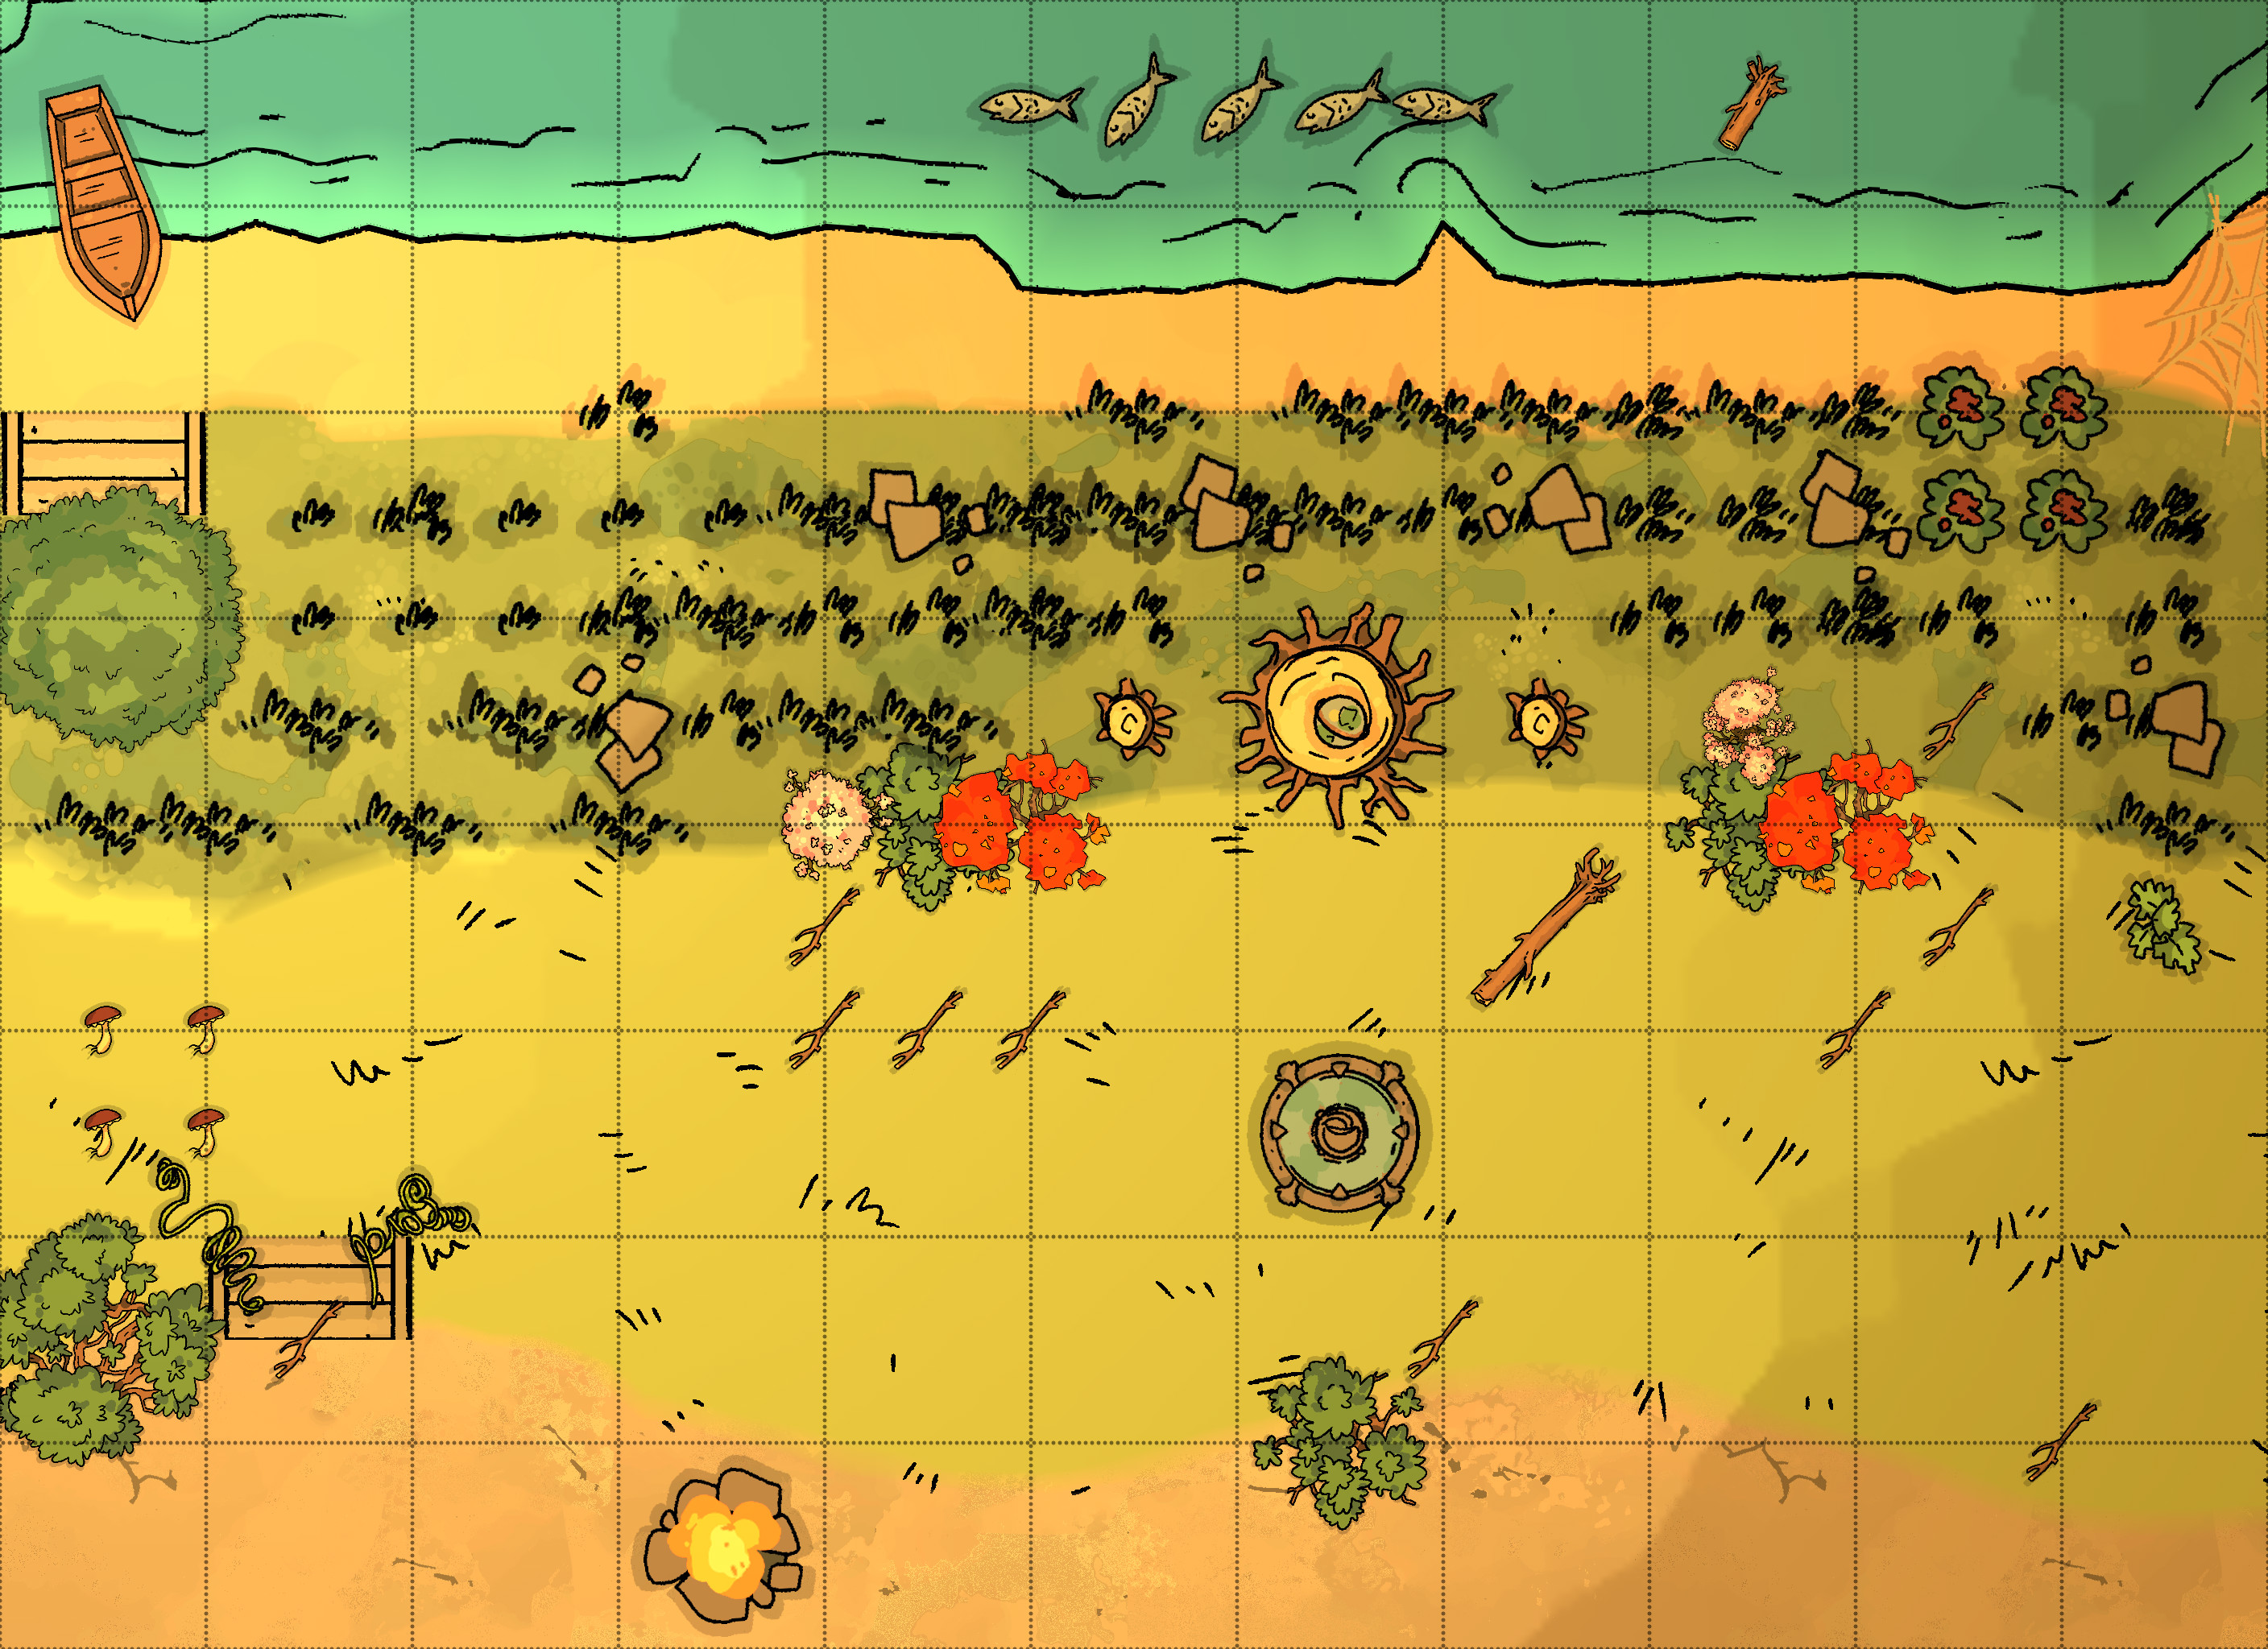
\includegraphics[height=1.1\textwidth, angle=90]{chap1.jpg}

\subsection{Background information}

(The default character is Clementine, who is a sneaky blue ninja living on earth.)

This adventure is built for one Level 1 Player Characters, you should scale the difficulty if there are more than one kid. This adventure is designed for new Players and Guides. It’s a great place to start if you’re
new to playing this game, there will be detailed record of what I did as a guide.

\subsection{Adventure Overview}

The player went to Lake Hudson for a stargazing, and they decide to do a camping that night. As the sun goes down, the moon starts to come out and the stars are showing their sneaky smiles. Suddenly, there is a comet coming down and hit the ground near the campsite. When the player go to the comet and check the interior, there is a blue dragon waiting for them, she seems wounded and weak, and she speaks the language that the player does not know.

The dragon, whose name is Icy, is actually a pilot of the spaceship which is seen as the comet. The spaceship had an engine problem and thus hits the ground. The dragon is in need of help as she is running out of water, and also hungry. Also, she wants to fix her spaceship as there are parts missing from the spaceship Glacial. The engine were actually broken because there were small alien slimes who likes to eat the engine so they took it away and hid it. You will have to search the beach, avoid or defeat the slime and take the engine back.

\subsection{Story}
``I really want to go see the stars!'' Said by little Moby, who is wearing a sunhat, a pair of sunglasses and a sundress, holding his special binoculars in hand. \\You signed, as you just sneakyly went to the Lake Hudson yesterday and saw the star alone. It was beautiful, but you really don't want to share the views. \\``I know, but Lake Hudson is kind of far. Let's do something different, we can do a wobbly dance!'' \\``We can camp there, and it is going to be fuuuuun!''

A camping? You reconcile the decision. You have not been camping for long time, and having to go camping is not that bad at all! Camping is so fun! You might need someone to drive, so you brought (the guide) to come with you, along with Moby, your pet dog, no one else knows what she was talking about except you.


\end{document}